\documentclass[11pt]{article}
\usepackage{graphicx}
\begin{document}
\noindent
ACID 
Atomicity\\
Consistency \implies parallel connections\\
Isolation\\
Durability\\
$RW \rightarrow Model \rightarrow  Table$\\
model needs to model realworld\\
\\
Entity must be uniquely identified by its attributes, not relation
\\
ER diagram has entity sets, relation sets, aggregates etc.\\
| unconstrained \\($A1_1$ INT REFERENCES ENT_1($A1_1$))\\
\\
primary key is a combination so can have both\\
can have more than one value from each entity\\
zero participation
\\
Ternary {doctors, prescribes, drugs}
\\
\\\\\\
|$>$ at most 1 key constraint \\(ENT1 INT PRIMARY KEY REFERENCES TABLE(ENT2))\\
$<NULL, 1423>$ is not necessary as it is already in the original table
\\
how to know that a student is supervised that is why we have not null\\
give me all the students (without knowing if they are supervised) can use a projection - sid - on the students table
\\\\
| $>$ with |\\
If ENT2 is not associated with any ENT1, it is not in $𝑅𝐸𝐿$. If it is associated with ENT1,then PRIMARY KEY constraint ensures it appears only once.\\
\\
$-> $ with $<-$\\
$A1_1$ INT PRIMARY KEY REFERENCES ENT_1($A1_1$), $A1_2$ INT UNIQUE NOT NULL \\REFERENCES ENT_2($A1_2$),\\\\
$=> $exactly one total participation + key\\
 each student must be supervised by exactly 1 prof.
 \\
 Foreign key occurs where u can merge into a table\\
$A1_1$ INT \textbf{NOT NULL} REFERENCES ENT_1($A1_1$),\\
$A1_2$ INT PRIMARY KEY REFERENCES ENT_2($A1_2$),\\
\\
== 1 or more 
\\
ISA \\
PRIMARY KEY REFERENCES
Every student can be identified by Sid, then undergraduates can graduates must also be identifiable by Sid
\\
Identity dependency\\
For a given city in a particular city\\
there can be multiple union city\\
combination to be a entity
explains the references stateID\\
need to remove all the cities from indiana before removing indiana
plus two addition delete statements\\
\\
every identity dependency need an existential dependency\\
know the party exist\\
need a primary key to use a primary key\\
Overlapping constraint 
On delete Cascade (to avoid violate constraints)
When to use aggregation\\
FOREIGN KEY ($A1_1, A1_2$) REFERENCES REL_1($A1_1, A1_2$)\\
\\
ENT1 = 20, ENT2 = 30
Minimum entries in relationship\\
ENT1 || $<>$ || 	ENT2  0\\
ENT1 $==> <> <$|| ENT2 20\\
ENT1 $==> <> $ || ENT2 20 \\
ENT1 ||$> <> <$|| ENT2 0 \\
\\\\
Maximum entries in relationship\\
ENT1 || $<>$ || 	 ENT2 20 x 30 = 600\\
ENT1 $==> <> <$|| ENT2 20 not enough to go around\\
ENT1 $==> <> $ ||  ENT2 20\\
ENT1 ||$> <> <$||  ENT2 20\\
\\
nullary all attributes are primary key\\
unary  association between an entity and its attributes\\ 
%4. violates key constraint due to pid\\
\\
Sometimes, a constraint forces us to have circular references.  In that case, there are several ways to solve this two of which are shown below:
\\
Completely break the circularity and ignore certain constraints.
If you wish, you can recover the circularity via ALTER TABLE.
\\
horse owned by people to participate in a race
\\\\
ISA\\ 
cannot be non covering\\
If there is one entity then it is redundant, need to capture part time does not need an office.
\\
\subsection*{Joins}\\
SELECT R.rname, R.area, S.price\\
FROM sells S NATURAL JOIN restaurants R\\
WHERE S.pizza = 'Funghi'\\
\\\\
SELECT R.rname, (SELECT area from restaurants WHERE S.area = R.area) , S.price\\
FROM sells \\
WHERE S.pizza = 'Funghi'\\\\
\subsection*{Aggregate}\\
If DISTINCT is not specified, it will only look at Non-NULL values\\
WHERE will remove rows before the computation\\
\\
SELECT R.rname\\
FROM restaurant \\
GROUP by R.rname\\
\\
If you do the stable sorting yourself,\\
it is like sorting col2 DESC before col1 ASC
\\
\\
Get normalized mean
\begin{verbatim}
SELECT SUM(y)  FROM (
 SELECT ((x - (SELECT MIN(x) + 0.0 FROM vals)) /
	 (SELECT MAX(x) + 0.0  - MIN(x) + 0.0 FROM vals))  
	 AS y FROM vals GROUP BY x) AS z
	 
is equivalent to 
SELECT (SUM(x)-COUNT(x)*MIN(x))/(MAX(x)-MIN(x)+0.0)
\end{verbatim}
Closed form formula = $\frac{sum_{x}(x_{i}) + sum_{x} (-min(X))}{max(X) - min(X)}$
\subsection*{Case analysis}
SELECT * FROM players\\
ORDER BY\\
 CASE WHEN title = 'Leader' THEN point END DESC,\\
 CASE WHEN title = 'Minion' THEN point END ASC\\
 which attribute to sort  (title = '')\\
 how to sort (ASC, DESC)\\
 \\
 scalar subqueries \leq 1 row, = 1 col, 0 \rightarrow NULL
 \\
  \subsection*{SQL EXCEPT}
  \begin{verbatim}

SELECT DISTINCT cname 
FROM likes
EXCEPT ALL
SELECT DISTINCT cname 
FROM likes
WHERE pizza IN (SELECT pizza FROM sells WHERE
rname = 'Corleone Corner');
  	
  \end{verbatim}
\\is equivalent to \\
   \begin{verbatim}

SELECT cname 
FROM likes
EXCEPT
SELECT cname 
FROM likes
WHERE pizza IN (SELECT pizza FROM sells WHERE
rname = 'Corleone Corner');
  	
  \end{verbatim}
  
  \subsection*{SQL EXISTS}
    \begin{verbatim}
SELECT DISTINCT cname 
FROM likes
EXCEPT ALL
SELECT DISTINCT cname 
FROM likes L
WHERE EXISTS (SELECT 1 FROM sells S WHERE
rname = 'Corleone Corner'
AND L.pizza = S.pizza);
    \end{verbatim}
  \subsection*{SQL ANY}
  \begin{verbatim}

SELECT DISTINCT name
FROM sells
WHERE rname <> 'C'
AND price > ANY (SELECT price FROM sells WHERE rname = 'C')

is equivalent to

SELECT DISTINCT s1.rname
FROM sells s1, sells s2
WHERE s1.price > s2.price AND s2.rname = 'Corleone Corner' 
AND s1.rname <> 'Corleone Corner'


Total order property
SELECT DISTINCT name
FROM sells
WHERE rname <> 'C'
AND price > (SELECT MIN(price) FROM sells WHERE rname = 'C')
    \end{verbatim}
    
    \subsection*{SQL ALL}
      $\pi_{rname, pizza, price} ( \sigma_{s1price > s2price)} (\rho_{(s1price, rname)}(sells)  \times \sigma_{(s2price, rname)}(sells) ))$
      \\\\
  \begin{verbatim}
SELECT DISTINCT rname, pizza, price
FROM sells S1
WHERE S1.price >= ALL (SELECT S2.price
FROM sells S2 
WHERE S1.rname = S2.rname)

    \end{verbatim}\\\\
 \subsection*{Scoping}
 ambiguous\\
 \\
SELECT *
FROM (SELECT * FROM sells) AS T,
(SELECT * FROM T) AS R
\\
\\
\subsection*{CTE}
\begin{verbatim}
	WITH intermediate AS
(SELECT C.cid, C.name, COUNT(*)
FROM enrolls E NATURAL JOIN courses C
GROUP BY C.cid)

SELECT name, num
FROM intermediate
WHERE num > (SELECT num FROM intermediate 
             WHERE name = "Database Systems"
            AND cid = 'CS2102');
            
WITH X AS ... WHERE a > 20
	 Y AS ... WHERE b < 10
	\end{verbatim} 
E.g. a not present cte
\begin{verbatim}
WITH 
not_present AS (
SELECT sid, week
FROM (SELECT sid FROM Students) AS tbl,
(SELECT DISTINCT week FROM presenters) AS wk_tbl
	
\end{verbatim}
\newpage
\subsection*{Where instead of having}
\begin{verbatim}
WITH CTE
SELECT COUNT(*)

SELECT FROM CTE
WHERE
\end{verbatim}

\subsection*{Consecutive values in a table}
Suppose n=3\\
q1 = not in table and max(n) > 3 \\
q2 = 4th onwards \\
q3 = max - n\\
q4 = between n and n - 3 - 1 \\
\\
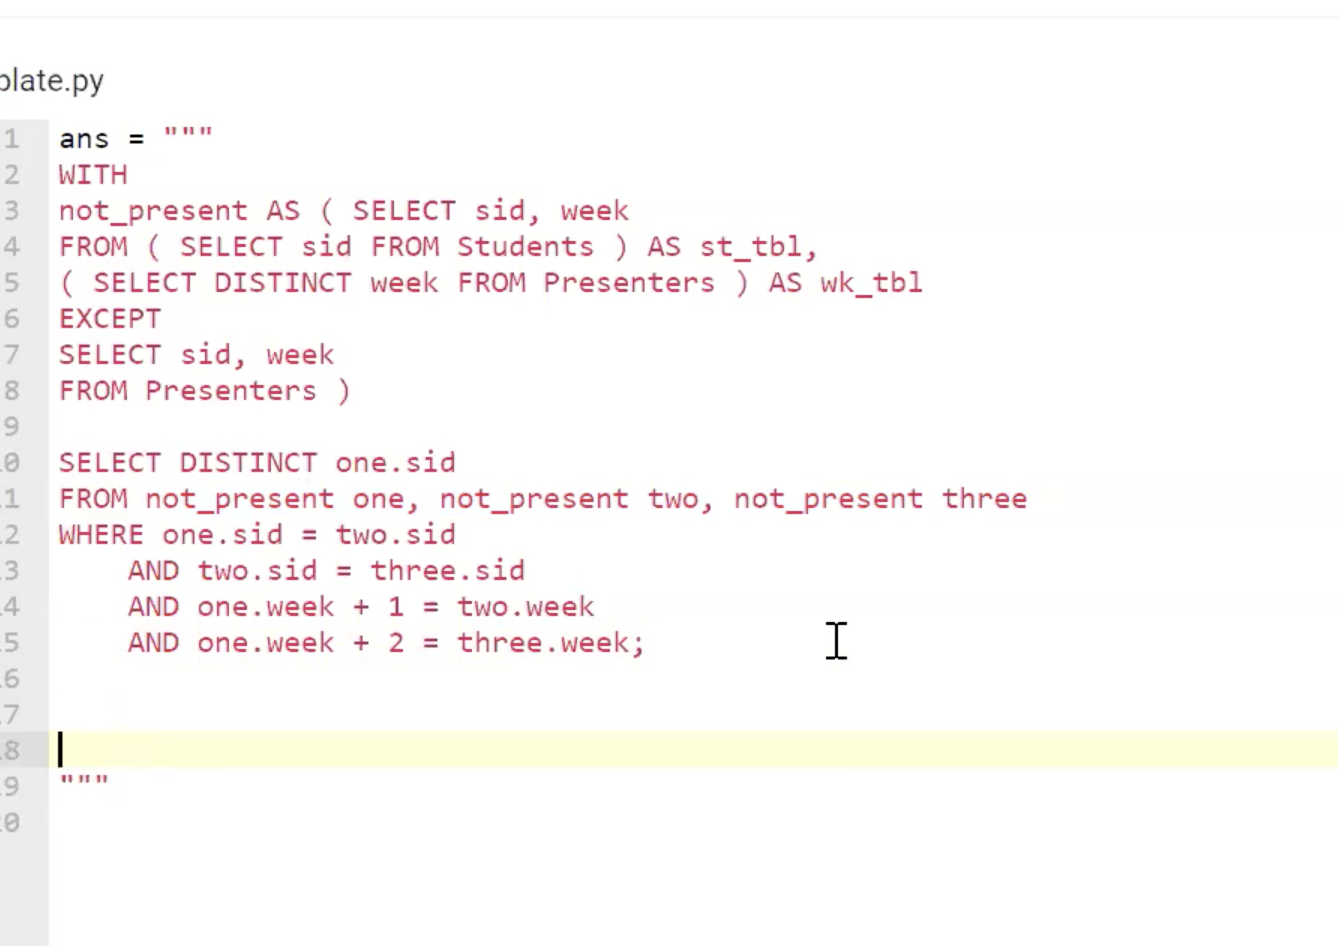
\includegraphics[height=7cm]{s.png}
\subsection*{Variables}
capturing a computation process
CTE: common table expression (temporary table unlike VIEW which is persistent)
\\
imperative, computes line by line, don't care how it is computed\\
E.g. SELECT * FROM $\_\_$ WHERE x is parent and x is male \\
\\
\\
Likes all pizza sold by a restaurant\\
If restaurants has pizza A and B\\
customers likes A, B, C\\
this subset should be still be included
\subsection*{Coalesce}
If there is no entry or is null, fill with 0\\
\begin{verbatim}
SELECT COALESCE(MIN(num), 0) FROM status;	
\end{verbatim}
\subsection*{Universal Quantification}
\textbf{Intuition}
\\
$|P_{1}| \geq |P_{2}| for \{1, 2, 3\} \not\subset \{4, 5\}$
$S1 \cup S = S1$ when S1 already contains S
$S1 \cap S$ = S
as they are incomparable
\\\\
\textbf{Double negation}
There is no pizza sold by CC where not (P likes pizza) 
\subsection*{Functional Dependencies}
\textbf{Reflexivity}\\
AB $\rightarrow$ A 
\\\\
\textbf{Composition}\\
A $\rightarrow$ B \\
C $\rightarrow$ D \\
AC $\rightarrow$ BD \\
\\
\\
\textbf{Logical implication}\\
Does it hold for all instances in the table
\\\\
If FD is R(A, B, C, D)\\
then total number of FDs is (2^4 - 1) $\times$  ($2^4$ - 1)\\
excluding itself so -1\\
\\
A $\rightarrow$ BC is also A $\rightarrow$ B and A $\rightarrow $C
\\\\
Attribute redundancy\\
AB $\rightarrow$ C and B $\rightarrow$ A
\\
We can replace AB $\rightarrow$ C with A $\rightarrow$ C
\\
\\
FD redundancy - remove without changing its meaning\\
A $\rightarrow$ B and B $\rightarrow$ C means A $\rightarrow$ C is redundant\\
For each FD, check for every single node on the destination and if there is a path from source to destination
\\
minimum cover is not unique
\\
\\
\textbf{How to get key}\\
If there is no arrow pointing to them in the hyper-graph, we need to include it as part of the key\\
\\
\textbf{How to get attribute closure}\\
For e.g. AD+ = ACDE\\\\

\includegraphics[height=4cm]{s1}
\\
Using the hyper-graph connect the source to the nodes at the left side of the implication\\
- Is there a path that can reach the nodes given at the right side of the implication
\\\\
\textbf{How to get minimal cover}\\
Usually the implications that can't be decomposed\\\\
Cannot have redundant attributes\\
AB $\rightarrow$ CDE\\
B+ check if B can determine CDE\\
which means A is redundant\\
B $\rightarrow$ CDE
\\\\
\textbf{How to get key}\\
\includegraphics[height=4cm]{s3.png}}
\\
Given a superkey
CDG+\\
Then try all combinations\\
CD+ CG+ DG+\\
Find attributes that is missing from the rhs
\subsection*{Decomposition}
Intuition is like splitting the relation into two or more\\\\
\textbf{Lossless join}\\\\
If the relation only contain attributes on RHS most likely it is not lossless
\\
$F \models (R1 \cap R2)$ satisfy a FD\\
1. Combine two relations into one\\
2. Each R can only be used one in the tree\\\\
\includegraphics[height=4cm]{images/s1.png}
\\\\
\textbf{Dependency preserving}\\
Cannot include anything that is trivial\\\\
As long it satisfy one of the attribute on LHS, then the FD is satisfied. Can use the output to another FD.\\\\
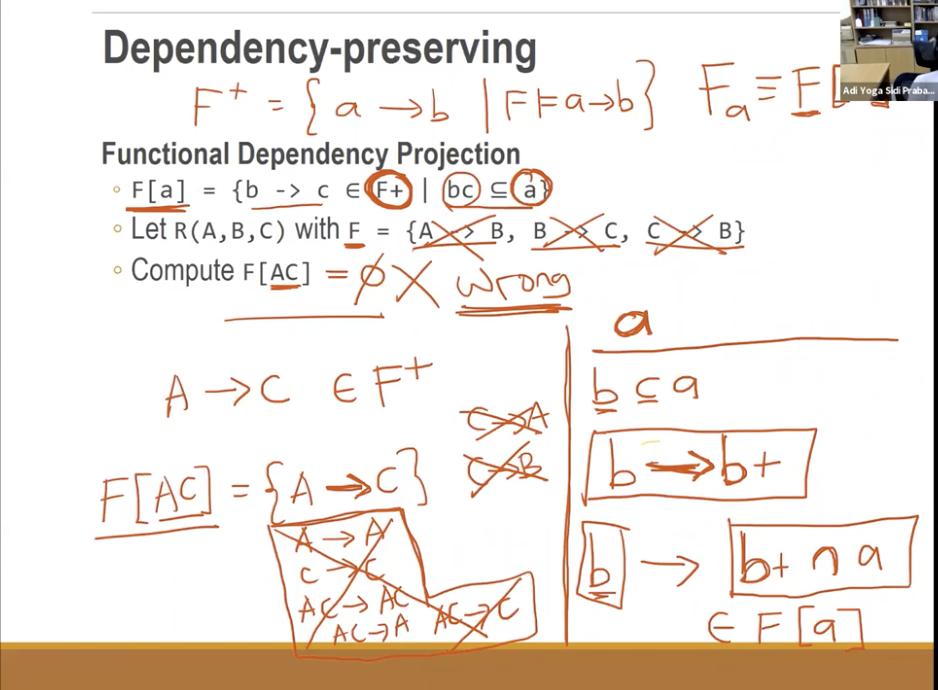
\includegraphics[height=5cm]{images/s2.png}
\\\\\\
Does R1 contain the attributes that is described by any FD?\\
\includegraphics[height=5cm]{images/s3.png}
\end{document}
